\chapter{Background}

\section{Domain Specific Languages}

A general-purpose programming language is designed for writing software in a variety of application domains. It is used by programmers to instruct computers by implementing any program that is computable by a Turing machine \cite{DslEngineering2013}. Conversely, a domain specific language is optimised for a given class of problems called a domain.  The syntax is based on abstractions that are closely aligned with the domain for which the language is built. A domain specific languages syntax is suitable for expressing these abstractions concisely \cite{DslEngineering2013}. A notable example of a domain specific language is Structured Query Language (SQL), designed for managing data held in a relational database management system. \newline \par

There are many advantages of using a domain specific language over a general-purpose language. The main advantage is that the domain specific language provides an additional layer of abstraction for the user. Notation can be defined that expresses the abstractions concisely and makes interacting with programs efficient and straightforward. This notation allows users of the domain specific language to have less experience with programming due to the limited scope of the language. It provides a clean level of abstraction that moves away from general-purpose languages and API’s which non-programmers are not competent enough to use. This abstraction allows non-programmers to work with a language closely aligned with the domain they work in \cite{DslEngineering2013},  yielding programs that are easy to understand, reason about, and maintain \cite{685738}. This is a crucial solution to the problem area as it abstracts the complexity of using API’s by creating a language which is syntactically simpler than a general-purpose language. \newline \par

Another advantage of using a domain specific language is their ability to be analysed and maintained. Due to the limited complexity of domain specific languages, certain properties such as termination can be determined, unlike general-purpose languages. These properties allow the domain specific language to be safer, often throwing less and more meaningful errors, which can be useful when dealing with critical services. For a domain specific language to execute it requires an interpreter or compiler.

\section{Interpreter}

For the execution and implementation of a language, another program or application is required to read the language and react to the phrases and input symbols it discovers. The program or application to execute this task is the interpreter. To execute the input, the interpreter must react to the valid sentences, phrases and sub-phrases of a particular language. The interpreter needs to be able to recognise phrases and identify the valid components of the phrase and differentiate it from other phrases \cite{parr2013definitive}. \newline \par

After the recognition of each phrase in a program, the interpreter will execute precompiled application specific code based on the phrase and valid components of the input \cite{hudak1997domain}. Unlike compilers, interpreters do not require code generation to machine language. Programs that recognise languages are called parsers, and this process is broken down into two stages, lexical analysis and parsing.

\section{Lexer}

Lexical analysers, often referred to as lexers, are programs which read the input stream of characters making up the source program, groups the characters into meaningful sequences called lexemes and produce as output a sequence of tokens for each lexeme \cite{aho2003compilers}. Tokens may be considered the building blocks of the language as it is more convenient to process a source program as a sequence of tokens rather than a string of characters. Tokens consist of two pieces of information, the token type, used to identify the lexical structure and the text matched for that token by the lexer in the form $\langle \textit{token-name}, \textit{attribute-value} \rangle$ \cite{aho2003compilers}. In general-purpose languages such as Java, examples of token types are int (integers), double (floating-point numbers). Another task the lexer performs is stripping out comments and white space in a source program.\newline \par

Lexers do not check the grammatical syntax of the language, as it will not check if the tokens are used in the wrong combination and will only produce a list of tokens. The list of tokens is passed to the subsequent phase, parsing, which is the process of identifying if an input is syntactically correct. 

\section{Parser}

A parser is a program to recognise the sentence structure of an input which is the process of structuring an input text according to a given grammar. The parser uses the token types of the tokens produced by the lexical analyser to produce a tree-like intermediate representation that depicts the grammatical structure of the token stream \cite{aho2003compilers}.

\subsection{Grammar}

A grammar is a formalism for describing the syntactic structure of programs in a programming language. A grammar describes how to form grammatical strings from a language's alphabet that are valid according to the syntax of the language by a set of production rules \cite{meduna2014formal}. A grammar derives strings by beginning with the start symbol and repeatedly replacing a nonterminal by the body of production for the nonterminal. The terminal strings that can be derived from the start symbol form the language defined by the grammar \cite{aho2003compilers}. A grammar does not describe the meaning of the strings in any given context and only describes their form.\newline \par

A context-free grammar is a grammar in which the left-hand side of every production rule consists of only a single nonterminal symbol in the form $ A \rightarrow \alpha$ where $A$ is a single nonterminal symbol, and $\alpha$ is a string of terminals and/or nonterminals \cite{aho1971translations}. A grammar is context-free when the production rules can be applied regardless of the context of a nonterminal. Since the semantics of a language is defined in terms of the syntax, the context-free-grammar is also instrumental in the definition of the semantics \cite{grune2012modern}. \newline \par

The formal definition of a context-free grammar G is defined by a four-tuple $G = (V, \varSigma, P, S)$, where $V$ and $\varSigma$ are disjoint finite sets of non-terminals and terminals which make up the content of the sentence \cite{aho1971translations}. $S$ is the start variable/symbol, used to represent the whole sentence or program and is an element of V. $P$ is a finite list of productions or rewrite rules of the form $ A \rightarrow \alpha$, where $A$ is in $V$ and $\alpha$ in $(V\cup\varSigma)^\ast$ \cite{backus1960report}.

\subsubsection{Left-recursive Grammar}

In a context-free grammar G, if there is a production in the form $X \rightarrow Xa$ where $X$ is a non-terminal and $a$ is a string of terminals, it is called a left recursive production. The grammar having a left recursive production is called a left recursive grammar, and this grammar would fall into infinite recursion when executed \cite{moore2000removing}.

\subsection{Parse Tree}

The parser will generate a syntax/parse tree which is a data structure that precisely shows how various segments of the program text and component phrases are to be recognised in terms of the grammar. Parse trees are a useful data structure as they contain complete information about how the parser grouped symbols into phrases and can easily be traversed by programmers \cite{parr2013definitive}. The construct of a parse-tree can be made by taking a derivational view, in which productions are treated as rewriting rules. The initiation of the derivation starts with the start symbol, and each rewriting step replaces a nonterminal by the body of one of its productions. An example of a parse tree is if a nonterminal $A$ has a production $A \rightarrow XYZ$, then a parse tree may have an interior node labelled A with three child nodes, labelled from left to right $X$, $Y$ and $Z$ \cite{aho2003compilers}. 

\begin{figure}[H]
  \centering
  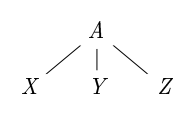
\includegraphics[width=0.25\textwidth]{images/parse-tree2.PNG}
  \caption{Example Parse tree \cite{aho2003compilers}}
\end{figure}

A formal definition of a parse tree according to a context-free grammar is a tree with the following properties \cite{aho2003compilers}:
\begin{itemize}
    \item The root node is labeled by the start symbol.
    \item Each leaf node is labeled by a terminal or by $\epsilon$.
    \item Each interior node is labeled by a nonterminal.
\end{itemize}

\begin{figure}[H]
  \centering
  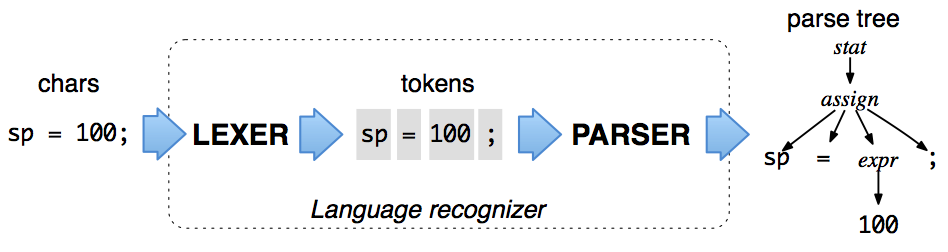
\includegraphics[width=1\textwidth]{images/antlr2.png}
  \caption{Data flow of a lexer and parser \cite{parr2013definitive}}
\end{figure}

\subsection{Top-down Parsing}

A top-down parser uses a context-free grammar $G$ and works on an input string $w$. It verifies that w is syntactically correct by constructing the derivation tree for $w$ in a top-down way. A derivation of an input for a grammar is a sequence of grammar rule applications that transform the start symbol into the string. The derivation proves that the input belongs to the language of the grammar. The derivation reads input string $w$ from left to right, and the parser starts at the tree node and proceeds down towards the frontier denoted by $w$. A LL grammar is a grammar that can be parsed by an LL parser. The first L stands for left-to-right scan of the input string $w$ and the second L means that the parser simulates the leftmost derivation of $w$ \cite{meduna2014formal}.